\documentclass[11pt,openany]{article}

\usepackage{mathtools, commath}
% Packages for formatting
\usepackage[margin=1in]{geometry}
\usepackage{fancyhdr}
\usepackage{enumerate}
\usepackage{graphicx}
\usepackage{kotex}
\usepackage{arydshln} % Include this package
\usepackage{bbding}
\usepackage{amsmath}
\usepackage{amsthm}
\usepackage[dvipsnames,table]{xcolor}
\usepackage{amssymb, amsfonts}
\usepackage{wasysym}
\usepackage{footnote}
\usepackage{tablefootnote}
\usepackage{arydshln} % Include this package
% Fonts
\usepackage[T1]{fontenc}
\usepackage[utf8]{inputenc}
\usepackage{newpxtext,newpxmath}
\usepackage{sectsty}

% Define colors
\definecolor{TealBlue1}{HTML}{0077c2}
\definecolor{TealBlue2}{HTML}{00a5e6}
\definecolor{TealBlue3}{HTML}{b3e0ff}
\definecolor{TealBlue4}{HTML}{00293c}
\definecolor{TealBlue5}{HTML}{e6f7ff}

\definecolor{thmcolor}{RGB}{231, 76, 60}
\definecolor{defcolor}{RGB}{52, 152, 219}
\definecolor{lemcolor}{RGB}{155, 89, 182}
\definecolor{corcolor}{RGB}{46, 204, 113}
\definecolor{procolor}{RGB}{241, 196, 15}

\usepackage{color,soul}
\usepackage{soul}
\newcommand{\mathcolorbox}[2]{\colorbox{#1}{$\displaystyle #2$}}
\usepackage{cancel}
\newcommand\crossout[3][black]{\renewcommand\CancelColor{\color{#1}}\cancelto{#2}{#3}}
\newcommand\ncrossout[2][black]{\renewcommand\CancelColor{\color{#1}}\cancel{#2}}

\usepackage{hyperref}
\usepackage{booktabs}

% Chapter formatting
\definecolor{titleTealBlue}{RGB}{0,53,128}
\usepackage{titlesec}
\titleformat{\section}
{\normalfont\sffamily\Large\bfseries\color{titleTealBlue!100!gray}}{\thesection}{1em}{}
\titleformat{\subsection}
{\normalfont\sffamily\large\bfseries\color{titleTealBlue!50!gray}}{\thesubsection}{1em}{}

%Tcolorbox
\usepackage[most]{tcolorbox}
\usepackage{multirow}
\usepackage{multicol}

\usepackage[linesnumbered,ruled]{algorithm2e}
\usepackage{algpseudocode}
\usepackage{setspace}
\SetKwComment{Comment}{/* }{ */}
\SetKwProg{Fn}{Function}{:}{end}
\SetKw{End}{end}
\SetKw{DownTo}{downto}

% Define a new environment for algorithms without line numbers
\newenvironment{algorithm2}[1][]{
	% Save the current state of the algorithm counter
	\newcounter{tempCounter}
	\setcounter{tempCounter}{\value{algocf}}
	% redefine the algorithm numbering (remove prefix)
	\renewcommand{\thealgocf}{}
	\begin{algorithm}
	}{
	\end{algorithm}
	% Restore the algorithm counter state
	\setcounter{algocf}{\value{tempCounter}}
}

\usepackage{adjustbox}
% Header and footer formatting
\pagestyle{fancy}
\fancyhead{}
\fancyhf{}
\rhead{\textcolor{TealBlue2}{\large\textbf{기대수(기초부터 대학원 수학까지 시리즈) 3기}}}%\rule{3cm}{0.4pt}}
\lhead{\textcolor{TealBlue2}{\large\textbf{수학의 즐거움, Enjoying Math}}}
% Define footer
%\newcommand{\footer}[1]{
%\begin{flushright}
%	\vspace{2em}
%	\includegraphics[width=2.5cm]{school_logo.jpg} \\
%	\vspace{1em}
%	\textcolor{TealBlue2}{\small\textbf{#1}}
%\end{flushright}
%}
%\rfoot{\large Department of Information Security, Cryptogrphy and Mathematics, Kookmin Uni.\includegraphics[height=1.5cm]{school_logo.jpg}}
\fancyfoot{}
\fancyfoot[C]{-\thepage-}

\usepackage{tcolorbox}
\tcbset{colback=white, arc=5pt}

\definecolor{axiomcolor}{HTML}{a88bfa}
\definecolor{defcolor}{RGB}{52, 152, 219}
\definecolor{procolor}{RGB}{241, 196, 15}
\definecolor{thmcolor}{RGB}{231, 76, 60}
\definecolor{lemcolor}{RGB}{155, 89, 182}
\definecolor{corcolor}{RGB}{46, 204, 113}
\definecolor{execolor}{RGB}{90, 128, 127}

% Define a new command for the custom tcolorbox
\newcommand{\axiombox}[2][]{%
	\begin{tcolorbox}[colframe=axiomcolor, title={\color{white}\bfseries #1}]
		#2
	\end{tcolorbox}
}

\newcommand{\defbox}[2][]{%
	\begin{tcolorbox}[colframe=defcolor, title={\color{white}\bfseries #1}]
		#2
	\end{tcolorbox}
}

\newcommand{\lembox}[2][]{%
	\begin{tcolorbox}[colframe=lemcolor, title={\color{white}\bfseries #1}]
		#2
	\end{tcolorbox}
}

\newcommand{\probox}[2][]{%
	\begin{tcolorbox}[colframe=procolor, title={\color{white}\bfseries #1}]
		#2
	\end{tcolorbox}
}

\newcommand{\thmbox}[2][]{%
	\begin{tcolorbox}[colframe=thmcolor, title={\color{white}\bfseries #1}]
		#2
	\end{tcolorbox}
}

\newcommand{\corbox}[2][]{%
	\begin{tcolorbox}[colframe=corcolor, title={\color{white}\bfseries #1}]
		#2
	\end{tcolorbox}
}



\usepackage{amsthm}

% Define custom theorem styles
\newtheoremstyle{dotless} % Name of the style
{3pt} % Space above
{3pt} % Space below
{\itshape} % Body font
{} % Indent amount
{\bfseries} % Theorem head font
{} % Punctuation after theorem head
{2.5mm} % Space after theorem head
{} % Theorem head spec

\newtheoremstyle{definitionstyle} % Name of the style
{3pt} % Space above
{3pt} % Space below
{} % Body font
{} % Indent amount
{\bfseries} % Theorem head font
{.} % Punctuation after theorem head
{2.5mm} % Space after theorem head
{} % Theorem head spec

% Applying custom styles
\theoremstyle{dotless}
\newtheorem{theorem}{Theorem} % Theorem environment with section-wise numbering
\newtheorem{proposition}[theorem]{Proposition} % Theorem environment with section-wise numbering
\newtheorem{lemma}[theorem]{Lemma} % Lemma shares the counter with theorem
\newtheorem{corollary}[theorem]{Corollary} % Corollary shares the counter with theorem

\theoremstyle{definitionstyle}
\newtheorem*{observation}{\textcolor{Magenta}{Observation}}
\newtheorem{definition}{Definition} % Definition shares the counter with theorem
\newtheorem{example}{Example} % Example shares the counter with theorem
\newtheorem{exercise}{Exercise} % Example shares the counter with theorem
\newtheorem{remark}{Remark} % Remark shares the counter with theorem
\newtheorem*{note}{Note}

\newtheorem*{definition*}{Definition} % Definition shares the counter with theorem
\newtheorem*{example*}{Example} % Example shares the counter with theorem
\newtheorem*{exercise*}{\textcolor{violet}{Exercise}} % Example shares the counter with theorem
\newtheorem*{remark*}{Remark} % Remark shares the counter with theorem


\usepackage{tikz}
\usepackage{tikz-cd}
\usepackage{tikz-3dplot}
\usepackage{pgfplots}
\pgfplotsset{compat=newest} % Adjust to your version of pgfplots
\def\Circlearrowleft{\ensuremath{%
		\rotatebox[origin=c]{180}{$\circlearrowleft$}}}
\def\Circlearrowright{\ensuremath{%
		\rotatebox[origin=c]{180}{$\circlearrowright$}}}
\def\CircleArrowleft{\ensuremath{%
		\reflectbox{\rotatebox[origin=c]{180}{$\circlearrowleft$}}}}
\def\CircleArrowright{\ensuremath{%
		\reflectbox{\rotatebox[origin=c]{180}{$\circlearrowright$}}}}
\usetikzlibrary{
	3d, % For 3D drawing
	angles,
	arrows,
	arrows.meta,
	backgrounds,
	bending,
	calc,
	decorations.pathmorphing,
	decorations.pathreplacing,
	decorations.markings,
	fit,
	matrix,
	patterns,
	patterns.meta,
	positioning,
	quotes,
	shadows,
	shapes,
	shapes.geometric,
	tikzmark
}
\tikzset{
	% single mid‐path arrow
	mid arrow/.style={
		decoration={
			markings,
			mark=at position 0.5 with {\arrow{Stealth[scale=1.2]}}
		},
		postaction={decorate},
	},
	% style for field arrows
	field arrow/.style={
		-{Stealth[scale=1.0]},
		thick,
		blue!70!black,
	},
}
\newcommand{\ie}{\textnormal{i.e.}}
\newcommand{\rsa}{\mathsf{RSA}}
\newcommand{\rsacrt}{\mathsf{RSA}\textendash\mathsf{CRT}}
\newcommand{\inv}[1]{#1^{-1}}

%New Command
%\newcommand{\set}[1]{\left\{#1\right\}}
\newcommand{\N}{\mathbb{N}}
\newcommand{\Z}{\mathbb{Z}}
\newcommand{\Q}{\mathbb{Q}}
\newcommand{\R}{\mathbb{R}}
\newcommand{\cR}{\mathcal{R}}
\newcommand{\C}{\mathbb{C}}
\newcommand{\F}{\mathbb{F}}
\newcommand{\nbhd}{\mathcal{N}}
\newcommand{\Log}{\operatorname{Log}}
\newcommand{\Arg}{\operatorname{Arg}}
\newcommand{\pv}{\operatorname{P.V.}}

\newcommand{\of}[1]{\left( #1 \right)} 
%\newcommand{\abs}[1]{\left\lvert #1 \right\rvert}
%\newcommand{\norm}[1]{\left\| #1 \right\|}

\newcommand{\sol}{\textcolor{magenta}{\bf Sol}}
\newcommand{\conjugate}[1]{\overline{#1}}

\newcommand{\res}{\operatorname{res}}
\DeclareMathOperator*{\Res}{\operatorname{Res}}

%\renewcommand{\Re}{\operatorname{Re}}
%\renewcommand{\Im}{\operatorname{Im}}

\newcommand{\cyclic}[1]{\langle #1 \rangle}
\newcommand{\uniform}{\overset{\$}{\leftarrow}}
\newcommand{\xmark}{\textcolor{red}{\XSolidBrush}}
\newcommand{\vmark}{\textcolor{green!75!black}{\CheckmarkBold}}

\newcommand{\gen}[1]{\langle #1 \rangle}
\newcommand{\Gen}[1]{\left\langle #1 \right\rangle}

\newcommand{\img}[1]{\text{Img}(#1)}
\newcommand{\Img}[1]{\text{Img}\left(#1\right)}
\newcommand{\preimg}[1]{\text{Img}^{-1}(#1)}
\newcommand{\Preimg}[1]{\text{Img}^{-1}\left(#1\right)}

\newcommand{\relation}{\mathrel{\mathcal{R}}}
\newcommand{\injection}{\rightarrowtail}
\newcommand{\surjection}{\twoheadrightarrow}
\newcommand{\id}{\textnormal{id}}

\newcommand{\eqclass}[1]{\left[#1\right]}

% Define custom colors for O and X
\newcommand{\yes}{\textcolor{blue}{\bf \fullmoon}}
\newcommand{\no}{\textcolor{red}{\bf \texttimes}}

\DeclarePairedDelimiter\ceil{\lceil}{\rceil}
\DeclarePairedDelimiter\floor{\lfloor}{\rfloor}
%\renewcommand{\floor}[#1]{\lfloor #1\rfloor}
%\newcommand{\Floor}[#1]{\left\lfloor #1\right\rfloor}
%\newcommand{\ceil}[#1]{\lceil #1\rceil}
%\newcommand{\Ceil}[#1]{\left\lceil #1\right\rceil}

\newcommand{\topology}{\mathscr{T}}
\newcommand{\sequence}[1]{\langle #1\rangle}
\renewcommand{\vec}[1]{\mathbf{#1}}
\setstretch{1.25}

%\usepackage{background}
%\backgroundsetup{
%	scale=3,
%	color=gray!20,
%	opacity=0.3,
%	angle=45,
%	contents={\Huge \sffamily Ji, Yong-hyeon}
%}
\begin{document}
\pagenumbering{arabic}
\begin{center}
	\huge\textbf{Linear Algebra II}\\
	\vspace{0.5em}
	\large{Ji, Yong-hyeon}\\
%	\large{\ttfamily \url{https://github.com/Hacker-Code-J}}\\
	\vspace{0.5em}
	\normalsize{\today}\\
\end{center}

\noindent 
We cover the following topics in this note.
\begin{itemize}
	\item Coordinate
	\item Linear Transformation
	\item Vector Space Isomorphism
	\item Classification of Vector Space (up to Isomorphism)
	\item Matrix Representation of a Linear Transformation
	\item TBA
\end{itemize}
\hrule\vspace{12pt}
%\tableofcontents
%\newpage
\vspace{20pt}
\begin{center}
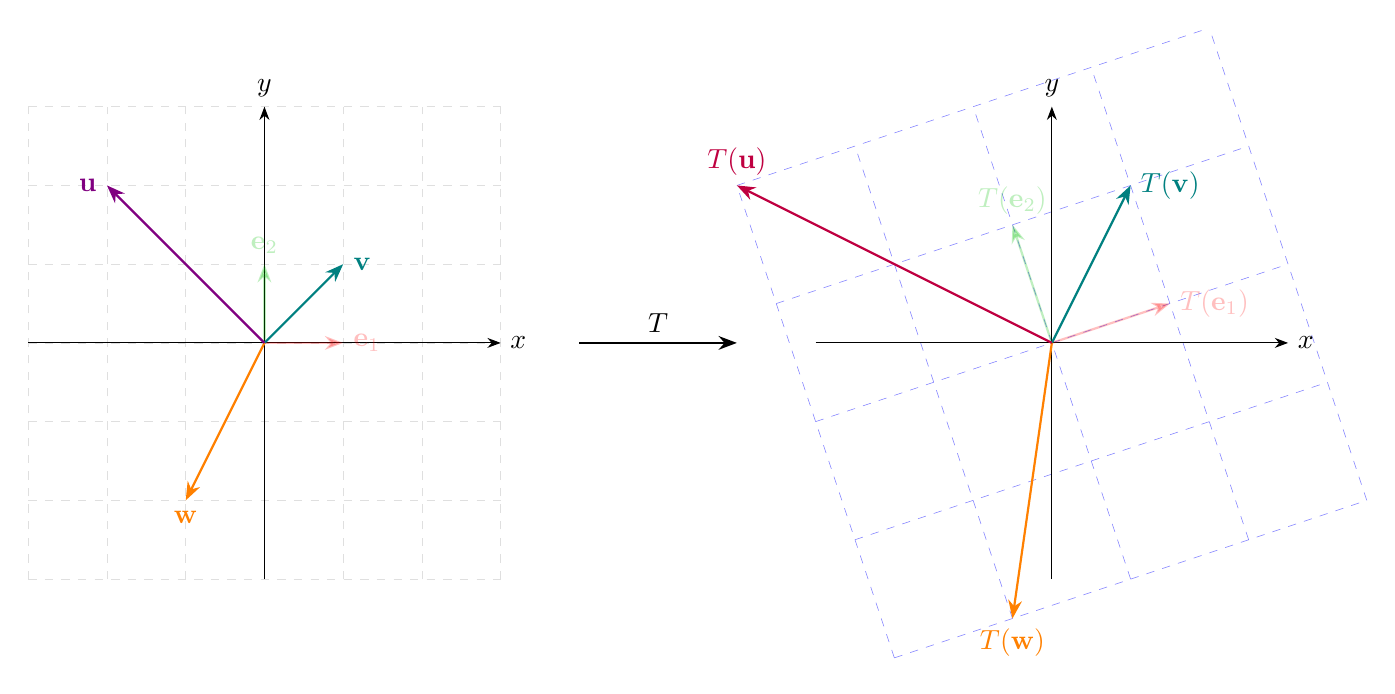
\begin{tikzpicture}[scale=1, >=Stealth]
	% Domain grid and vectors
	\begin{scope}
		% Draw the domain grid
		\draw[step=1, gray!50, very thin, dashed, opacity=.5] (-3,-3) grid (3,3);
		\draw[->] (-3,0) -- (3,0) node[right] {$x$};
		\draw[->] (0,-3) -- (0,3) node[above] {$y$};
		
		% Draw basis vectors in the domain
		\draw[->, red, thick, opacity=.25] (0,0) -- (1,0) node[anchor=west] {$\mathbf{e}_1$};
		\draw[->, green!75!black, thick, opacity=.25] (0,0) -- (0,1) node[anchor=south] {$\mathbf{e}_2$};
		
		% A sample vector in the domain, for example, v = (1,1)
		\draw[->, teal, thick] (0,0) -- (1,1) node[anchor=west] {$\mathbf{v}$};
		\draw[->, orange, thick] (0,0) -- (-1,-2) node[anchor=north] {$\mathbf{w}$};
		\draw[->, violet, thick] (0,0) -- (-2,2) node[anchor=east] {$\mathbf{u}$};
	\end{scope}
	
	% Arrow indicating the transformation from Domain to Codomain
	\draw[->, thick] (4,0) -- (6,0) node[midway, above] {$T$};
	
	% Codomain (transformed grid and vectors)
	\begin{scope}[shift={(10,0)}]
		% Draw the transformed grid by applying the transformation matrix T:
		% T = [1.5  -0.5; 0.5  1.5]
		\begin{scope}[cm={1.5,0.5,-0.5,1.5,(0,0)}]
			\draw[step=1, blue, very thin, dashed, opacity=.5] (-2,-2) grid (2,2);
		\end{scope}
	
		% Draw the codomain axes
		\draw[->] (-3,0) -- (3,0) node[right] {$x$};
		\draw[->] (0,-3) -- (0,3) node[above] {$y$};
		
		% Draw transformed basis vectors:
		% T(e1) = (1.5, 0.5)
		\draw[->, red, thick, opacity=.25] (0,0) -- (1.5,0.5) node[anchor=west] {$T(\mathbf{e}_1)$};
		% T(e2) = (-0.5, 1.5)
		\draw[->, green!75!black, thick, opacity=.25] (0,0) -- (-0.5,1.5) node[anchor=south] {$T(\mathbf{e}_2)$};
		
		% Draw the transformed sample vector:
		% T(1,1) = T(e1+e2) = T(e1)+T(e2) = (1.5-0.5, 0.5+1.5) = (1,2)
		\draw[->, teal, thick] (0,0) -- (1,2) node[anchor=west] {$T(\mathbf{v})$};
		\draw[->, orange, thick] (0,0) -- (-.5,-3.5) node[anchor=north] {$T(\mathbf{w})$};
		\draw[->, purple, thick] (0,0) -- (-4,2) node[anchor=south] {$T(\mathbf{u})$};
	\end{scope}
\end{tikzpicture}
\end{center}

\newpage
\probox[Uniqueness of Representation with respect to a Basis]{\begin{proposition*}\hypertarget{unique-wrt-basis}{
	Let \( V \) be a vector space over a field \( \F \) and let $\dim V=n<\infty$. Let
	\[
	\basis=\set{\vec{b}_1, \vec{b}_2, \dots, \vec{b}_n }\subseteq V
	\]
	be a basis of \( V \). Then for every vector \( \vec{v} \in V \) there exists a unique scalars \(\alpha_1, \alpha_2, \dots, \alpha_n \in \F\) such that
	\[
	\vec{v} = \alpha_1\vec{b}_1 + \alpha_2\vec{b}_2+\cdots+\alpha_n\vec{b}_n = \sum_{i=1}^{n} \alpha_i\, \vec{b}_i.
	\]}
\end{proposition*}}

\begin{proof}
	Suppose, for contradiction, that there exist two distinct representations of some vector \( \vec{v} \in V \) in terms of the basis \( \basis=\set{\vec{b}_1,\vec{b}_2,\dots,\vec{b}_n} \):
	\[
	\vec{v} = \sum_{i=1}^{n} \alpha_i\, \vec{b}_i \quad \text{and} \quad \vec{v} = \sum_{j=1}^{n} \beta_j\, \vec{b}_j,
	\]
	where \(\alpha_i, \beta_j \in \F\) for all \( i, j \). Then \begin{align*}
		\sum_{i=1}^{n} \alpha_i\, \vec{b}_i - \sum_{j=1}^{n} \beta_j\, \vec{b}_j = \vec{0}\implies
		\sum_{i=1}^{n} (\alpha_i-\beta_i)\, \vec{b}_i= \vec{0}.
	\end{align*} Since a basis $\basis=\set{\vec{b}_1,\vec{b}_2,\dots,\vec{b}_n}$ is linearly independent, we have \[
	\alpha_i-\beta_i=0,\quad\ie,\quad \alpha_i=\beta_i
	\] for all $i=1,2,\dots,n$. 
	Therefore, the representation of any \( \vec{v} \in V \) as a finite linear combination of elements of the basis \( \basis \) is unique.
\end{proof}
\vfill
\newpage
\defbox[Coordinate in a Finite-Dimensional Vector Space]{\begin{definition*}
Let \(V\) be a vector space over a field \(\F\) with $\dim V=n<\infty$, and let  
\[
\basis = \{\vec{b}_i\}_{i=1}^n=\set{\vec{b}_1,\vec{b}_2,\dots,\vec{b}_n}
\]
be a basis of \(V\). The \hl{\textbf{coordinate of $\vec{v}\in V$ with respect to $\basis$}}, denoted by \([\vec{v}]_\basis\), is the \(n\)-tuple
\[
[\vec{v}]_\basis = (\alpha_1,\alpha_2,\dots,\alpha_n) \quad \text{where } \vec{v} = \alpha_1 \vec{b}_1 + \alpha_2 \vec{b}_2 + \cdots + \alpha_n \vec{b}_n.
\]
\end{definition*}}\vspace{20pt}
{\color{gray!30}\begin{remark*}[Coordinate Function]
%In the general case (possibly infinite-dimensional), the coordinates are given by the unique function \( [\vec{v}]_\basis \) assigning to each basis vector \(\vec{b}\) the scalar coefficient in the unique representation of \(\vec{v}\).
Let \( V \) be a vector space over a field \( \F \) and let $\basis = \{ \vec{b}_i \}_{i \in I}$
be a (Hamel) basis for \( V \). Then for every vector \( \vec{v} \in V \), there exists a unique function
\[
[\vec{v}]_\basis : \basis \to \F
\]
with the finite set \( S=\{\, \vec{b} \in \basis : [\vec{v}]_\basis(\vec{b}) \neq 0 \,\} \) such that $\abs{S}<\infty$ and 
\[
\vec{v} = \sum_{\vec{b} \in \basis} [\vec{v}]_\basis(\vec{b})\ \vec{b}.
\]
The function \([\vec{v}]_\basis\) is called the \textit{coordinates of \( \vec{v} \) with respect to the basis \( \basis \)}. In the finite-dimensional case where $\basis = \{\vec{b}_1, \vec{b}_2, \dots, \vec{b}_n\},$
the coordinate function \([\vec{v}]_\basis\) is naturally identified with the \( n \)-tuple
\[
[\vec{v}]_\basis = (\alpha_1, \alpha_2, \dots, \alpha_n) \quad \text{where} \quad \vec{v} = \alpha_1 \vec{b}_1 + \alpha_2 \vec{b}_2 + \cdots + \alpha_n \vec{b}_n.
\] 
Furthermore, the mapping \[
\Phi:V\to \F^\basis,\quad \vec{v}\mapsto[\vec{v}]_\basis.
\] is a vector space isomorphism, which assigns to each $\vec{v}\in V$ its coordinate vector w.r.t. the basis $\basis$.
\end{remark*}}
\vfill
\newpage
\begin{observation}
\ \begin{center}
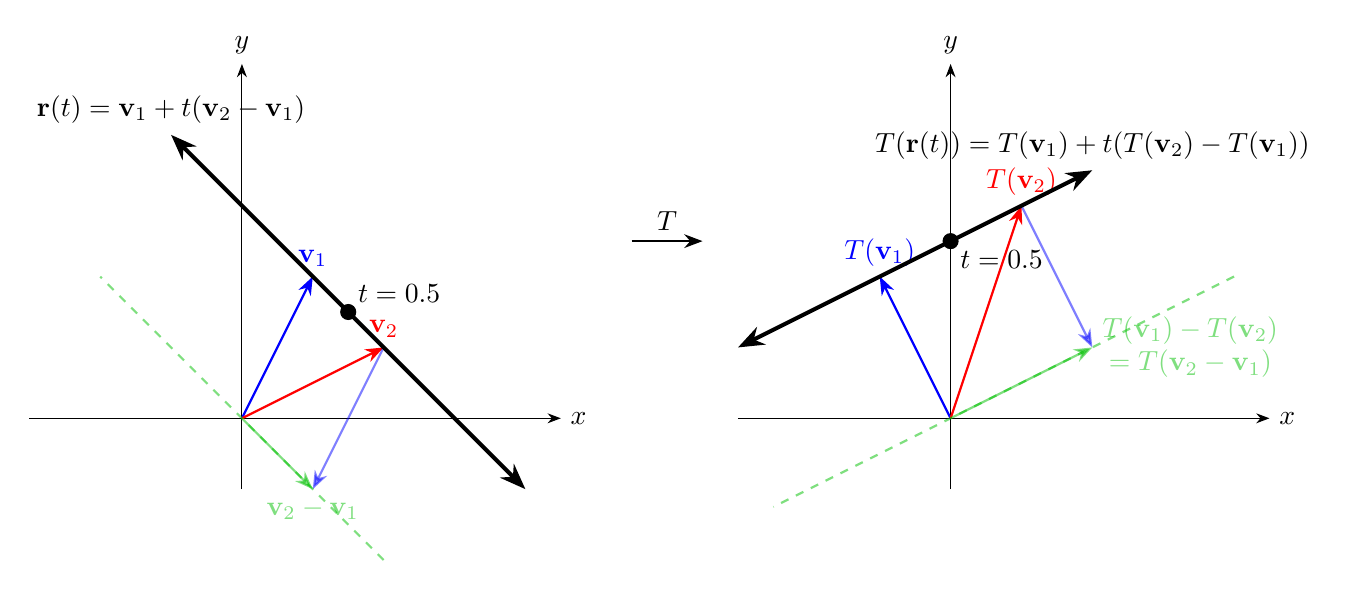
\begin{tikzpicture}[scale=.9, >=Stealth]
	\begin{scope}[shift={(0,0)}]
		% Draw coordinate axes for the domain
		\draw[->] (-3,0) -- (4.5,0) node[right] {$x$};
		\draw[->] (0,-1) -- (0,5) node[above] {$y$};
		
		% Define vectors v1 and v2 exactly:
		\coordinate (v1) at (1,2);   % v1 = (1,1)
		\coordinate (v2) at (2,1);   % v2 = (4,2)
		
		% Draw v1 and v2
		\draw[->, thick, blue] (0,0) -- (v1) node[above] {$\vec{v}_1$};
		\draw[->, thick, red] (0,0) -- (v2) node[above] {$\vec{v}_2$};v2
		\draw[->, thick, blue, opacity=.5] (v2) -- (1,-1) node[above] {};
		\draw[-, dashed, thick, green!75!black, opacity=.5] (2,-2) -- (-2,2) node[above] {};
		\draw[->, thick, green!75!black, opacity=.5] (0,0) -- (1,-1) node[below] {$\vec{v}_2-\vec{v}_1$};
		
		% Draw the line: r(t)=v1+t*(v2-v1) with t from -1 to 2.
		% For t=-2: r(-1)=(1,2)-2*(1,-1)=(-1,4).
		% For t=-1: r(-1)=(1,2)-1*(1,-1)=(0,3).
		% For t=0: r(0)=(1,2)-1*(1,-1)=(1,2).
		% For t=1.25: r(1.25)=(1,2)+1.5*(1,-1)=(2.5,0.5).
		% For t=2: r(2)=(1,2)+2*(1,-1)=(3,0).
		% For t=3: r(3)=(1,2)+3*(1,-1)=(4,-1).
		\coordinate (A) at (-1,4);
		\coordinate (B) at (4,-1);
		\draw[<->, line width=.5mm] (B) -- (A) node[above] 
		{$\vec{r}(t)=\vec{v}_1+t(\vec{v}_2-\vec{v}_1)$};
		
		% Mark an accurately calculated point on the line for t=0.5:
		% r(0.5)=(1,2)+0.5*(1,-1)=(1.5,1.5)
		\coordinate (p) at (1.5,1.5);
		\filldraw (p) circle (3pt) node[above right] {$t=0.5$};
	\end{scope}
	
	\draw[->, thick] (5.5,2.5) -- (6.5,2.5) node[midway, above] {$T$};
	
	\begin{scope}[shift={(10,0)}]
		% Draw coordinate axes for the domain
	\draw[->] (-3,0) -- (4.5,0) node[right] {$x$};
	\draw[->] (0,-1) -- (0,5) node[above] {$y$};
	
	% Define vectors v1 and v2 exactly:
	\coordinate (Tv1) at (-1,2);   % v1 = (1,1)
	\coordinate (Tv2) at (1,3);   % v2 = (4,2)
	
	% Draw v1 and v2
	\draw[->, thick, blue] (0,0) -- (Tv1) node[above] {$T(\vec{v}_1)$};
	\draw[->, thick, red] (0,0) -- (Tv2) node[above] {$T(\vec{v}_2)$};v2
	\draw[->, thick, blue, opacity=.5] (Tv2) -- (2,1) node[above] {};
	\draw[-, dashed, thick, green!75!black, opacity=.5] (4,2) -- (-2.5,-1.25) node[above] {};
	\draw[->, thick, green!75!black, opacity=.5] (0,0) -- (2,1) node[right, align=center] {$T(\vec{v}_1)-T(\vec{v}_2)$\\ $=T(\vec{v}_2-\vec{v}_1)$};
	
	% Draw the line: T(r(t))=Tv1+t*T(v2-v1) with t from -1 to 2.
	% For t=-1: r(-1)=(-1,2)-1*(2,1)=(-3,1).
	% For t=1.5: r(2)=(-1,2)+1.5*(2,1)=(2,3.5).
	% For t=2: r(2)=(-1,2)+2*(2,1)=(3,4).
	\coordinate (A) at (-3,1);
	\coordinate (B) at (2,3.5);
	\draw[<->, line width=.5mm] (A) -- (B) node[above] 
	{$T(\vec{r}(t))=T(\vec{v}_1)+t(T(\vec{v}_2)-T(\vec{v}_1))$};
	
	% Mark an accurately calculated point on the line for t=0.5:
	% r(0.5)=(-1,2)+0.5*(2,1)=(0,2.5)
	\coordinate (p) at (0,2.5);
	\filldraw (p) circle (3pt) node[below right] {$t=0.5$};
	\end{scope}
\end{tikzpicture}
\end{center}
\end{observation}\vspace{20pt}
\defbox[$\star$ Linear Transformation $\star$]{\begin{definition*}
	Let $V$ and $W$ be vector spaces over a field $\F$. A function \[
	T:V\to W
	\] is called a \textbf{linear transformation} if for all vectors $\vec{v}_1,\vec{v}_2\in V$ and for all scalars $\alpha,\beta\in \F$, the following condition holds: \[
	T(\alpha\vec{v}_1+\beta\vec{v}_2)=\alpha T(\vec{v}_1)+\beta T(\vec{v}_2).
	\]
\end{definition*}}\vspace{20pt}
\begin{remark*}
	Equivalently, a function $T:V\to W$ is linear if it satisfies \begin{enumerate}[(i)]
		\item (\textit{Additivity}) For all $\vec{v}_1,\vec{v}_2\in V$, \[
		T(\vec{v}_1+\vec{v}_2)=T(\vec{v}_1)+T(\vec{v}_2);
		\]
		\item (\textit{Homogeneity}) For all $\alpha\in \F$ and $\vec{v}\in V$, \[
		T(\alpha\vec{v})=\alpha T(\vec{v}).
		\]
	\end{enumerate} 
\end{remark*}
\begin{remark*}
	This definition ensures $T$ preserves the vector space structure of $V$ in its image in $W$.
\end{remark*}

\newpage
\defbox[Vector Space Isomorphism]{\begin{definition*}
	Let $V$ and $W$ be vector spaces over a field $\F$. A mapping \[
	T:V\to W
	\] is called a \textbf{vector space isomorphism} if it satisfies the following conditions: \begin{enumerate}[(i)]
		\item (\textit{Linearity}) For any vectors $\vec{v}_2,\vec{v}_2\in V$ and any scalars $\alpha,\beta\in \F$, \[
		T(\alpha\vec{v}_1+\beta\vec{v}_2)=\alpha T(\vec{v}_1)+\beta T(\vec{v}_2).
		\]
		\item (\textit{Bijectivity})
		\begin{itemize}
			\item (\textit{Injectivity}) $\forall \vec{v}_1,\vec{v}_2\in V$,\ $T(\vec{v}_1)=T(\vec{v}_2)\implies\vec{v}_1=\vec{v}_2$;
			\item (\textit{Surjectivity}) $\forall \vec{w}\in W$,\ $\exists \vec{v}\in V$ such that $T(\vec{v})=\vec{w}$.
		\end{itemize}
	\end{enumerate} The bijectivity of $T$ guarantees the existence of an inverse mapping $T^{-1}:W\to V$, which satisfies \[
	(\forall \vec{v}\in V,\ T^{-1}(T(\vec{v}))=\vec{v}),\quad\text{and}\quad (\forall \vec{w}\in W,\ T(T^{-1}(\vec{w}))=\vec{w}).
	\]
\end{definition*}}
\begin{remark*}
	The inverse mapping $T^{-1}:W\to V$ is also a linear transformation.
	\begin{proof}
		Let $\vec{w}_1,\vec{w}_2\in W$ and let $\alpha,\beta\in \F$. Since $T$ is bijective, for each $\vec{w}\in W$, there exists a unique $\vec{v}\in V$ such that $\vec{w}=T(\vec{v})$. Define \[
		\vec{v}_1=T^{-1}(\vec{w}_1)\in V\quad\text{and}\quad\vec{v}_2=T^{-1}(\vec{w}_2)\in V.
		\] Since $T$ is linear, we have \[
		T(\alpha\vec{v}_1+\beta\vec{v}_2)=\alpha T(\vec{v}_1)+\beta T(\vec{v}_2)=\alpha\vec{w}_1+\beta\vec{w}_2.
		\] Thus, \begin{align*}
			T^{-1}(\alpha\vec{w}_1+\beta\vec{w}_2)&=T^{-1}(T(\alpha\vec{v}_1+\beta\vec{v}_2))\\
			&=\alpha\vec{v}_1+\beta\vec{v}_2\\
			&=\alpha T^{-1}(\vec{w}_1) + \beta T^{-1}(\vec{w}_2). 
		\end{align*}
	\end{proof}
\end{remark*}
\begin{remark*}
	When a vector space isomorphism $T:V\to W$ exists, the vector spaces $V$ and $W$ are said to be \textbf{isomorphic}, denoted by $V\simeq W$.
\end{remark*}

\newpage
\lembox{\begin{lemma*}\hypertarget{prop}{
	Let $V$ and $W$ be vector spaces over a field $\F$ with $\dim V<\infty$ and $\dim W<\infty$. The following are equivalent: \begin{enumerate}[(1)]
		\item $\dim V=\dim W$
		\item There exists a vector space isomorphism $T$ from $V$ to $W$
	\end{enumerate}}
\end{lemma*}}
\begin{proof}
\begin{enumerate}[]
	\item $((2)\Rightarrow (1))$ Assume that there exists a \textcolor{red}{vector space isomorphism} $T:V\to W$. Let $\basis_V=\set{\vec{v}_1,\vec{v}_2,\dots,\vec{v}_n}$ be any basis of $V$. Consider the set \[
	\img{\basis_V}=T[\basis_V]=\set{T(\vec{v}):\vec{v}\in \basis_V}=\set{T(\vec{v}_1),T(\vec{v}_2),\dots,T(\vec{v}_n)}\subseteq W.
	\] We claim that $T[\basis_V]$ is a basis of $W$: \begin{itemize}
		\item (\textit{Linear Independence}) Suppose that for some finite scalars $\set{\alpha_i}_{i=1}^n\subseteq \F$ we have \[
		\alpha_1T(\vec{v}_1)+\alpha_2T(\vec{v}_2)+\cdots+\alpha_nT(\vec{v}_n)=\vec{0}_W.
		\] By the \textcolor{red}{linearity} of $T$, we obtain $T(\alpha_1\vec{v}_1+\alpha_2\vec{v}_2+\cdots+\alpha_n\vec{v}_n)=\vec{0}_W$. Note that $T(\vec{0}_V)=T(0\cdot\vec{v})=0\cdot T(\vec{v})=\vec{0}_W$ for any $\vec{v}\in V$. Since $T$ is \textcolor{red}{injective}, it follows that \[
		\alpha_1\vec{v}_1+\alpha_2\vec{v}_2+\cdots+\alpha_n\vec{v}_n=\vec{0}_V.
		\] As $\basis_V=\set{\vec{v}_1,\vec{v}_2,\dots,\vec{v}_n}$ is a basis (and hence linearly independent), $\alpha_1=\alpha_2=\cdots=\alpha_n=0$. Thus, $T[\basis_V]$ is linearly independent.
		\item (\textit{Spanning Property}) Let $\vec{w}\in W$. Since $T$ is \textcolor{red}{surjective}, there exists $\vec{v}\in V$ such that \[
		T(\vec{v})=\vec{w}.
		\] By \hyperlink{unique-wrt-basis}{Uniqueness of Representation w.r.t. a Basis}, we know that there exists a unique scalars $\set{\alpha}_{i=1}^n\subseteq \F$ such that \[
		\vec{v}=\alpha_1\vec{v}_1+\alpha_2\vec{v}_2+\cdots\alpha_n\vec{v}_n.
		\] Then \[
		\vec{w}=T(\vec{v})=T(\alpha_1\vec{v}_1+\alpha_2\vec{v}_2+\cdots\alpha_n\vec{v}_n)\overset{\text{linearity}}{=}\alpha_1 T(\vec{v}_1)+\alpha_2 T(\vec{v}_2) + \cdots +\alpha_n T(\vec{v}_n)\in \Span T[\basis_V].
		\] That is, $\vec{w}\in W$ is a linear combination of elements of $T[\basis_V]$. Therefore, $\Span T[\basis_V]=W$.
	\end{itemize} Since $
	\abs[1]{\basis_V}=\abs[1]{T[\basis_V]}=n$, thus, we have \[
	\dim V=\dim W.
	\]
	\item $((1)\Rightarrow (2))$  Conversely, assume that $\dim V=\dim W =:n.$ Consider bases \[
	\basis_V=\set{\vec{v}_1,\vec{v}_2,\dots,\vec{v}_n}\quad\text{and}\quad\basis_W=\set{\vec{w}_1,\vec{w}_2,\dots,\vec{w}_n}
	\] for $V$ and $W$, respectively. By \hyperlink{unique-wrt-basis}{Uniqueness of Representation w.r.t. a Basis}, for each vector $\vec{v}\in V$, there exists a unique finite scalars $\set{\alpha_i}_{i=1}^n\subseteq \F$ such that \[
	\vec{v}=\alpha_1\vec{v}_1+\alpha_2\vec{v}_2+\cdots+\alpha_n\vec{v}_n.
	\] Define a mapping \[
	T:V\to W,\quad \vec{v}\mapsto T(\vec{v})=T\left(\sum_{i=1}^n\alpha_i\vec{v}_i\right):=\sum_{j=1}^n\alpha_j\vec{w}_j.
	\] for each $\vec{v}\in V$. We NTS that $T$ be a one-to-one and onto linear transformation: \begin{enumerate}[(i)]
		\item (\textit{Linearity}) Let $\vec{v},\vec{v}'\in V$ with $\vec{v}=\sum_{i=1}^n\alpha_i\vec{v}_i$ and $\vec{v}'=\sum_{j=1}^n\beta_j\vec{v}_j$. For any $\lambda,\mu\in\F$, we have \begin{align*}
		\lambda\vec{v}+\mu\vec{v}'=\lambda\sum_{i=1}^{n}\alpha_i\vec{v}_i+\mu\sum_{j=1}^{n}\beta_j\vec{v}_j
		&=\lambda(\alpha_1\vec{v}_1+\alpha_2\vec{v}_2+\cdots+\alpha_n\vec{v}_n)+\mu(\beta_1\vec{v}_1+\beta_2\vec{v}_2+\cdots+\beta_n\vec{v}_n)\\
		&=(\lambda\alpha_1+\mu\beta_1)\vec{v}_1+(\lambda\alpha_2+\mu\beta_2)\vec{v}_2+\cdots+(\lambda\alpha_n+\mu\beta_n)\vec{v}_n\\
		&=\sum_{k=1}^{n}\gamma_k\vec{v}_k\quad\text{where}\quad\gamma_k=
		\lambda\alpha_k+\mu\beta_k.
		\end{align*} By definition of $T$, we have \[
		T(\lambda\vec{v}+\mu\vec{v}')=\sum_{k=1}^{n}\gamma_k\vec{w}_k=\lambda\sum_{i=1}^{n}\alpha_i\vec{w}_i+\mu\sum_{j=1}^{n}\beta_j\vec{w}_j=\lambda T(\vec{v})+\mu T(\vec{v}').
		\]\vspace{20pt}
		\item (\textit{Injectivity}) Let $\vec{v},\vec{v}'\in V$ with $\vec{v}=\sum_{i=1}^n\alpha_i\vec{v}_i$ and $\vec{v}'=\sum_{j=1}^n\beta_j\vec{v}_j$. Suppose $T(\vec{v})=T(\vec{v}')$. Then \[
		T(\vec{v})-T(\vec{v}')=\sum_{k=1}^{n}\gamma_k\vec{w}_k=\vec{0}_W,\quad\text{where}\ \gamma_k=\alpha_k-\beta_k.
		\] Since $\basis_W=\set{\vec{w}_1,\vec{w}_2,\dots,\vec{w}_n}$ is a basis of $W$, the linear independence of $\basis_W$ implies that\[
		\alpha_k=\beta_k
		\] for all $k=1,2,\dots,n$. Thus $\vec{v}=\vec{v}'$, and so $T$ is injective. 
		\newpage
		\item (\textit{Surjectivity}) Let $\vec{w}\in W$. Since $\basis_W=\set{\vec{w}_1,\vec{w}_2,\dots,\vec{w}_n}$ is a basis of $W$, there exists a unique finite scalars $\set{\alpha_i}_{i=1}^n\subseteq \F$ such that \[
		\vec{w}=\alpha_1\vec{w}_1+\alpha_2\vec{w}_2+\cdots+\alpha_n\vec{w}_n.
		\] Define a vector \[
		\vec{v}:=\alpha_1\vec{v}_1+\alpha_2\vec{v}_2+\cdots+\alpha_n\vec{v}_n=\sum_{i=1}^n\alpha_i\vec{v}_i\in V.
		\] Then $T(\vec{v})=\sum_{i=1}^n\alpha_i\vec{w}_i=\vec{w}$. Thus, $T$ is surjective.
	\end{enumerate}
\end{enumerate}
\end{proof}
\thmbox[Classification of Vector Spaces up to Isomorphism]{\begin{theorem*}
	Let \[
	\mathcal{V}_\F:=\set{V:\text{$V$ is a vector space over a field $\F$}}.
	\] Define a relation $\sim$ on $\mathcal{V}_\F$ by \[
	\forall V,W\in\mathcal{V}_\F,\quad V\sim W\iff \exists T\in W^V\quad\text{such that}\quad\text{$T$ is a vector space isomorphism}.
	\] Then \begin{enumerate}[(1)]
		\item $\sim$ is an equivalence relation on $\mathcal{V}_\F$;
		\item $\forall V,W\in\mathcal{V}_\F$,\ $
		V\simeq W\iff \dim V=\dim W.$
	\end{enumerate}
	The isomorphism classes of vector spaces over $\F$ are completely determined by their dimensions.
\end{theorem*}}
\begin{proof}
\ \begin{enumerate}[(1)]
	\item We NTS that the relation $\sim$ is reflexive, symmetric, and transitive: \begin{enumerate}[(i)]
		\item (\textit{Reflexivity})\ For each $V\in\mathcal{V}_\F$, the identity map $\id_V:V\to V$ is a linear isomorphism, so $V\sim V$.
		\item (\textit{Symmetry})\ If $V\sim W$ via an isomorphism $T:V\to W$, then its inverse $T^{-1}:W\to V$ is also linear, implying $W\sim V$.
		\item (\textit{Transitivity})\ If $V\sim W$ via $T:V\to W$ and $W\sim U$ via $S:W\to U$, then the composition $S\circ T:V\to U$ is a linear isomorphism, so $V\sim U$.
	\end{enumerate}
	\item It is proved by \hyperlink{prop}{previous lemma}.
\end{enumerate}
\end{proof}
\corbox[Coordinate Isomorphism]{\begin{corollary*}
	Let $V$ be a vector space over a field $\F$ with $\dim V=n\in\N$, and let \[
	\F^n=\set{(x_1,x_2,\dots,x_n):x_i\in F,\ 1\leq i\leq n}
	\] is the space of $n$-tuples over $\F$ equipped with the usual operations of vector addition and scalar multiplication. . Then there exists a vector space isomorphism \[
	\Phi:V\to \F^n,\quad \ie,\quad V\simeq \F^n.
	\]
\end{corollary*}}
\begin{example*}
	Consider the vector space \[
	\text{Mat}_{n\times m}(\R)=\set{\begin{bmatrix}
			a_{11} & a_{12} & \cdots & a_{1m} \\
			a_{21} & a_{22} & \cdots & a_{2m} \\
			\vdots & \vdots & \ddots & \vdots \\
			a_{n1} & a_{n2} & \cdots & a_{nm}
		\end{bmatrix}: a_{ij}\in\R,\; 1\leq i\leq n,\; 1\leq j\leq m}
	\] which consists of all \( n \times m \) matrices with entries in \(\mathbb{R}\) (and where the vector space structure is defined over the field \(\mathbb{R}\)). Also, let \[
	\R^{nm}=\set{(x_1,x_2,\dots,x_{nm}):x_k\in \R,\; 1\leq k\leq nm}
	\] the vector space of \( nm \)-tuples of real numbers, with the usual coordinate-wise addition and scalar multiplication (again, over the field \(\mathbb{R}\)). Then there exists a vector space isomorphism \[
	\Phi : \operatorname{Mat}_{n \times m}(\mathbb{R}) \to \mathbb{R}^{nm},
	\] \ie, $\text{Mat}_{n\times m}(\R)\simeq \R^{nm}$.
%**Proof.**
%
%1. **Definition of the Mapping \(\Phi\).**
%
%For each matrix
%\[
%A = (a_{ij})_{1\le i\le n,\;1\le j\le m} \in \operatorname{Mat}_{n \times m}(\mathbb{R}),
%\]
%define the mapping
%\[
%\Phi(A) \coloneqq (a_{11},\, a_{12},\, \dots,\, a_{1m},\, a_{21},\, a_{22},\, \dots,\, a_{2m},\, \dots,\, a_{n1},\, a_{n2},\, \dots,\, a_{nm}) \in \mathbb{R}^{nm}.
%\]
%Here, the entries of \(A\) are arranged in a fixed order (e.g., row-major order).
%
%2. **Well-Definedness.**
%
%Since every matrix \(A \in \operatorname{Mat}_{n \times m}(\mathbb{R})\) has uniquely determined entries \(a_{ij} \in \mathbb{R}\), the ordered \(nm\)-tuple \(\Phi(A)\) is uniquely determined. Thus, \(\Phi\) is well-defined as a function from \(\operatorname{Mat}_{n \times m}(\mathbb{R})\) to \(\mathbb{R}^{nm}\).
%
%3. **Linearity of \(\Phi\).**
%
%We verify that \(\Phi\) preserves addition and scalar multiplication over \(\mathbb{R}\).
%
%- **Additivity:**  
%Let \(A = (a_{ij})\) and \(B = (b_{ij})\) be arbitrary matrices in \(\operatorname{Mat}_{n \times m}(\mathbb{R})\). Then
%\[
%A + B = (a_{ij} + b_{ij}),
%\]
%so
%\[
%\Phi(A+B) = (a_{11}+b_{11},\, a_{12}+b_{12},\, \dots,\, a_{nm}+b_{nm}).
%\]
%On the other hand,
%\[
%\Phi(A) + \Phi(B) = (a_{11},\, a_{12},\, \dots,\, a_{nm}) + (b_{11},\, b_{12},\, \dots,\, b_{nm}) = (a_{11}+b_{11},\, a_{12}+b_{12},\, \dots,\, a_{nm}+b_{nm}).
%\]
%Therefore,
%\[
%\Phi(A+B) = \Phi(A) + \Phi(B).
%\]
%
%- **Homogeneity:**  
%Let \(\lambda \in \mathbb{R}\) and \(A = (a_{ij})\). Then
%\[
%\lambda A = (\lambda a_{ij}),
%\]
%and thus
%\[
%\Phi(\lambda A) = (\lambda a_{11},\, \lambda a_{12},\, \dots,\, \lambda a_{nm}) = \lambda (a_{11},\, a_{12},\, \dots,\, a_{nm}) = \lambda\, \Phi(A).
%\]
%
%Consequently, \(\Phi\) is \(\mathbb{R}\)-linear:
%\[
%\forall\, A,B \in \operatorname{Mat}_{n \times m}(\mathbb{R}),\; \forall\, \lambda \in \mathbb{R},\quad \Phi(A+B) = \Phi(A) + \Phi(B) \quad \text{and} \quad \Phi(\lambda A) = \lambda\, \Phi(A).
%\]
%
%4. **Injectivity of \(\Phi\).**
%
%Assume \(A, B \in \operatorname{Mat}_{n \times m}(\mathbb{R})\) such that
%\[
%\Phi(A) = \Phi(B).
%\]
%Then,
%\[
%(a_{11},\, a_{12},\, \dots,\, a_{nm}) = (b_{11},\, b_{12},\, \dots,\, b_{nm}).
%\]
%This equality implies that
%\[
%a_{ij} = b_{ij} \quad \text{for all } 1 \le i \le n \text{ and } 1 \le j \le m.
%\]
%Hence, \(A = B\), which shows that \(\Phi\) is injective.
%
%5. **Surjectivity of \(\Phi\).**
%
%Let
%\[
%x = (x_1,x_2,\dots,x_{nm}) \in \mathbb{R}^{nm}
%\]
%be arbitrary. We need to find a matrix \(A \in \operatorname{Mat}_{n \times m}(\mathbb{R})\) such that \(\Phi(A) = x\). Define the matrix \(A = (a_{ij})\) by
%\[
%a_{ij} \coloneqq x_{(i-1)m + j}, \quad \text{for } 1 \le i \le n \text{ and } 1 \le j \le m.
%\]
%With this definition, the entries of \(A\) arranged in row-major order are exactly the coordinates of \(x\); that is,
%\[
%\Phi(A) = (x_1,x_2,\dots,x_{nm}) = x.
%\]
%Therefore, \(\Phi\) is surjective.
%
%6. **Conclusion.**
%
%Since \(\Phi : \operatorname{Mat}_{n \times m}(\mathbb{R}) \to \mathbb{R}^{nm}\) is a linear transformation that is both injective and surjective, it is an isomorphism of \(\mathbb{R}\)-vector spaces. Thus,
%\[
%\operatorname{Mat}_{n \times m}(\mathbb{R}) \cong \mathbb{R}^{nm}.
%\]
%
%\(\Box\)

\end{example*}
\vspace{20pt}
\begin{note}
We also denote the set of all $n\times m$ matrices with real entries, namely $\text{Mat}_{n\times m}(\R)$ by $\R^{n\times m}$.
\end{note}	

\newpage
\begin{observation}
	Let $V$ and $W$ be vector spaces over a field $\F$, and let $T:V\to W$ be a linear transformation. Suppose that \[
	\basis_V=\set{\vec{v}_1,\vec{v}_2,\dots,\vec{v}_n}\quad\text{and}\quad\basis_W=\set{\vec{w}_1,\vec{w}_2,\dots,\vec{w}_m}
	\] are bases for $V$ and $W$, respectively. Then for each $1\leq j\leq n$, there exist unique scalars $\set{a_{ij}}_{i=1}^m\subseteq \F$ such that $
	T(\vec{v}_j)=a_{1j}\vec{w}_1+a_{2j}\vec{w}_2+\cdots+a_{mj}\vec{w}_m$:
	\begin{center}\vspace{40pt}
	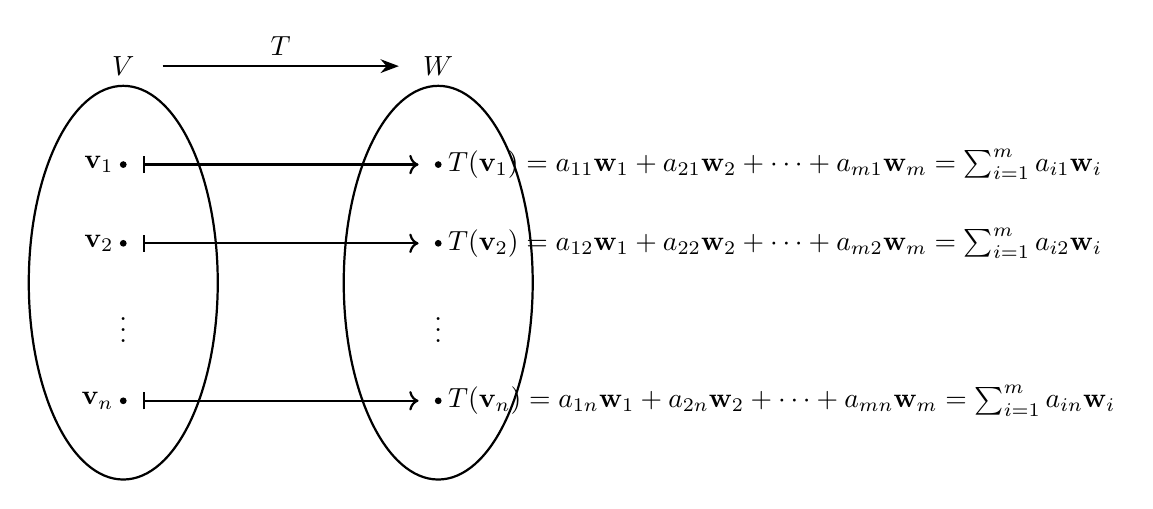
\begin{tikzpicture}
		% Draw the vector spaces V and W
		\draw[thick] (-2,0) ellipse (1.2 and 2.5); \node at (-2, 2.75) {$V$};
		\draw[thick] (2,0) ellipse (1.2 and 2.5); \node at (2, 2.75) {$W$};
		
		% Draw the arrows representing the function
		\draw[-Stealth, thick] (-1.5, 2.75) -- (1.5,2.75) node[midway, above] {$T$};
		
		\filldraw (-2,1.5) circle (1pt) node[left] {$\vec{v}_1$};
		\filldraw (2,1.5) circle (1pt) node[right] {$T(\vec{v}_1)=a_{11}\vec{w}_1+a_{21}\vec{w}_2+\cdots+a_{m1}\vec{w}_m=\sum_{i=1}^{m}a_{i1}\vec{w}_i$};
		\draw[|->, thick] (-1.75, 1.5) -- (1.75, 1.5);
		
		\filldraw (-2,.5) circle (1pt) node[left] {$\vec{v}_2$};
		\filldraw (2,.5) circle (1pt) node[right] {$T(\vec{v}_2)=a_{12}\vec{w}_1+a_{22}\vec{w}_2+\cdots+a_{m2}\vec{w}_m=\sum_{i=1}^{m}a_{i2}\vec{w}_i$};
		\draw[|->, thick] (-1.75, .5) -- (1.75, .5);
		
		\node at (-2,-.5) {$\vdots$};
		\node at (2,-.5) {$\vdots$};
		
		\filldraw (-2,-1.5) circle (1pt) node[left] {$\vec{v}_n$};
		\filldraw (2,-1.5) circle (1pt) node[right] {$T(\vec{v}_n)=a_{1n}\vec{w}_1+a_{2n}\vec{w}_2+\cdots+a_{mn}\vec{w}_m=\sum_{i=1}^{m}a_{in}\vec{w}_i$};
		\draw[|->, thick] (-1.75, -1.5) -- (1.75, -1.5);
	\end{tikzpicture}
	\end{center}\vspace{40pt}
	In other words, the action of $T$ on the basis of $V$ is completely determined by the matrix \[
	[T]_{\basis_V}^{\basis_W}:=\begin{bmatrix}
		: & : & & : \\
		T(\vec{v}_1)& T(\vec{v}_2) & \cdots & T(\vec{v}_n)\\
		: & : & & :
	\end{bmatrix}=\begin{bmatrix}
		a_{11} & a_{21} & \cdots & a_{1n}\\
		a_{21} & a_{22} & \cdots & a_{2n}\\
		\vdots & \vdots & \ddots &\vdots  \\
		a_{m1} & a_{m1} & \cdots & a_{mn}\\
	\end{bmatrix}\in\text{Mat}_{m\times n}(\F).
	\]
\end{observation}
%\vfill
\newpage
\begin{example*}
Consider the linear transformation \[
T:\R^2\to\R^2,\quad T(x,y)=(2x,0.5y).
\] Its effect on the standard basis vectors is \[
T(\vec{e}_1)=T(1,0)=(2,0)\quad\text{and}\quad T(\vec{e}_2)=T(0,1)=(0,0.5).
\]
\begin{center}
\begin{minipage}{.49\textwidth}
Then, we have 
\begin{align*}
T(x,y)&=(2x,\,0.5y)\\
&=\begin{bmatrix}
	: & : \\
	T(\vec{e}_1) & T(\vec{e}_2) \\
	: & : \\
\end{bmatrix}\begin{bmatrix}
	x \\ y
\end{bmatrix}=\begin{bmatrix}
	2 & 0 \\ 1 & 0.5
\end{bmatrix}\begin{bmatrix}
	x \\ y
\end{bmatrix}
\end{align*}
\end{minipage}\hfill
\begin{minipage}{.49\textwidth}
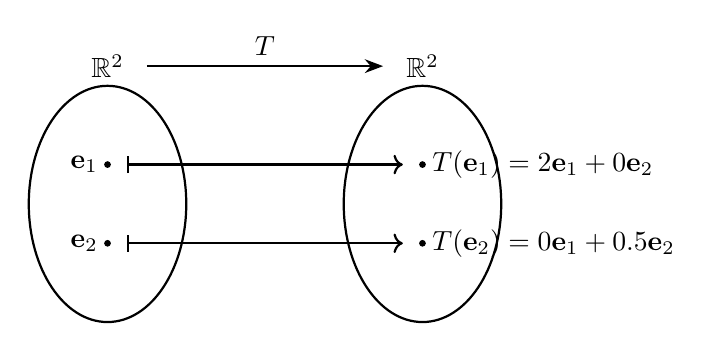
\begin{tikzpicture}
	% Draw the vector spaces V and W
	\draw[thick] (-2,0) ellipse (1 and 1.5); \node at (-2, 1.75) {$\R^2$};
	\draw[thick] (2,0) ellipse (1 and 1.5); \node at (2, 1.75) {$\R^2$};
	
	% Draw the arrows representing the function
	\draw[-Stealth, thick] (-1.5, 1.75) -- (1.5,1.75) node[midway, above] {$T$};
	
	\filldraw (-2,.5) circle (1pt) node[left] {$\vec{e}_1$};
	\filldraw (2,.5) circle (1pt) node[right, align=left] {$T(\vec{e}_1)=2\vec{e}_1+0\vec{e}_2$};
	\draw[|->, thick] (-1.75, .5) -- (1.75, .5);
	
	\filldraw (-2,-.5) circle (1pt) node[left] {$\vec{e}_2$};
	\filldraw (2,-.5) circle (1pt) node[right, align=left] {$T(\vec{e}_2)=0\vec{e}_1+0.5\vec{e}_2$};
	\draw[|->, thick] (-1.75, -.5) -- (1.75, -.5);
\end{tikzpicture}
\end{minipage}
\end{center}
\vfill
\begin{center}
	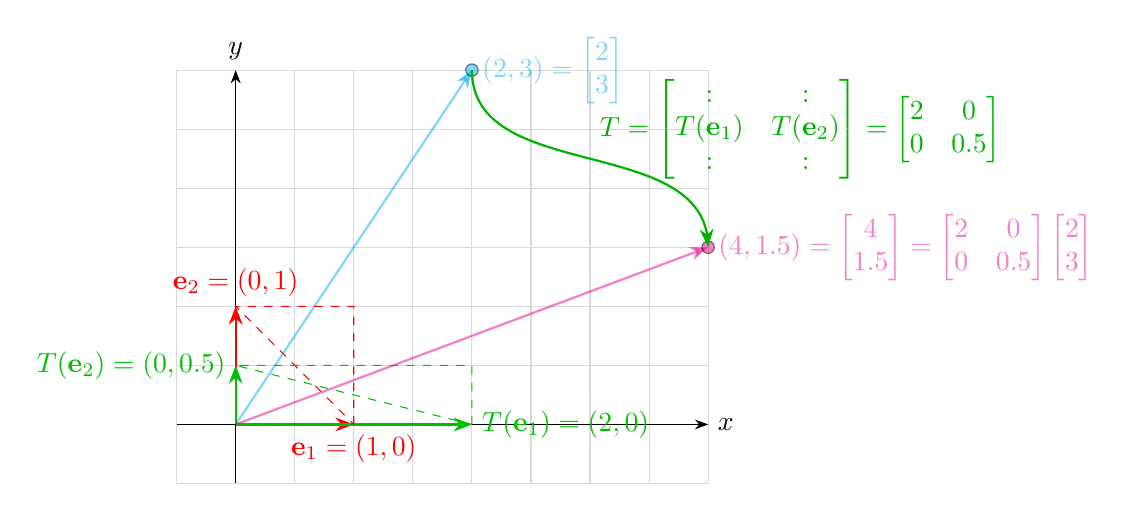
\begin{tikzpicture}[scale=1.5, >=Stealth]
	\foreach \x in {-.5,0,...,4}
	\draw[gray!30] (\x,-.5) -- (\x,3);
	\foreach \y in {-.5,0,...,3}
	\draw[gray!30] (-.5,\y) -- (4,\y);
	% Draw coordinate axes
	\draw[->] (-.5,0) -- (4,0) node[right] {$x$};
	\draw[->] (0,-.5) -- (0,3) node[above] {$y$};
	
	% Original standard basis vectors (blue)
	\draw[->,red,thick] (0,0) -- (1,0) node[below] {$\vec{e}_1=(1,0)$};
	\draw[->,red,thick] (0,0) -- (0,1) node[above] {$\vec{e}_2=(0,1)$};
	
	\draw[->,cyan,thick, opacity=.5] (0,0) -- (2,3) node[right] {$(2,3)=\begin{bmatrix}
			2\\ 3
		\end{bmatrix}$};
	
	% Transformed basis vectors under T (red)
	\draw[->,green!75!black,thick] (0,0) -- (2,0) node[right] {$T(\vec{e}_1)=(2,0)$};
	\draw[->,green!75!black,thick] (0,0) -- (0,0.5) node[left] {$T(\vec{e}_2)=(0,0.5)$};
	
	\draw[->,magenta,thick, opacity=.5] (0,0) -- (4,1.5) node[right] {$(4,1.5)=\begin{bmatrix}
			4 \\ 1.5
		\end{bmatrix}=\begin{bmatrix}
		2 & 0 \\ 0 & 0.5
	\end{bmatrix}\begin{bmatrix}
	2 \\ 3
\end{bmatrix}$};
	
	\draw[dashed, red] (1,0) -- (1,1) -- (0,1) -- cycle;
	\draw[dashed, green!75!black] (2,0) -- (2,0.5) -- (0,0.5) -- cycle;
	
	\draw[fill=cyan, opacity=.5] (2,3) circle (1.5pt);
	\draw[fill=magenta, opacity=.5] (4,1.5) circle (1.5pt);
	
	\draw[->, bend angle=45, green!70!black, out=-90, in=90, thick] (2,3) to (4,1.5);
	\node[right, green!70!black] at (3,2.5) {$T=\begin{bmatrix}
			\text{\string:} & \text{\string:} \\
			T(\vec{e}_1) & T(\vec{e}_2) \\
			\text{\string:} & \text{\string:} \\
		\end{bmatrix}=\begin{bmatrix}
			2 & 0 \\ 0 & 0.5
		\end{bmatrix}$};
\end{tikzpicture}
\end{center}
\vfill
\begin{center}
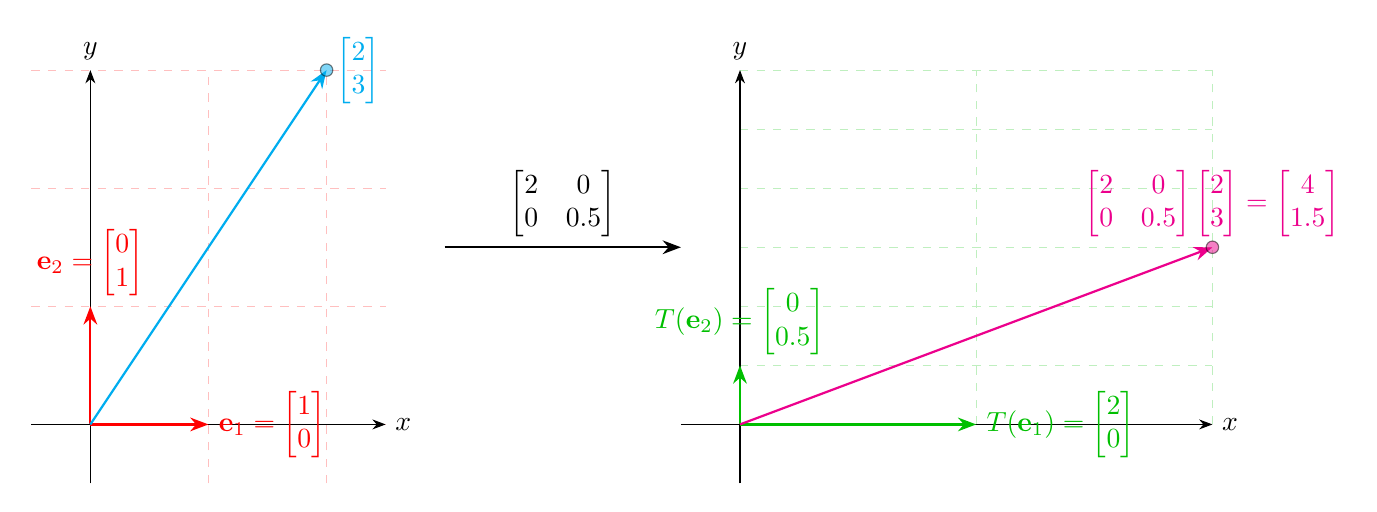
\begin{tikzpicture}[scale=1.5, >=Stealth]
\begin{scope}
	\draw[step=1, red, very thin, dashed, opacity=.25] (-.5,-.5) grid (2.5,3);
	\draw[->] (-.5,0) -- (2.5,0) node[right] {$x$};
	\draw[->] (0,-.5) -- (0,3) node[above] {$y$};
	
	% Draw basis vectors in the domain
	\draw[->, red, thick] (0,0) -- (1,0) node[anchor=west] {$\mathbf{e}_1=\begin{bmatrix}
			1 \\ 0
		\end{bmatrix}$};
	\draw[->, red, thick] (0,0) -- (0,1) node[anchor=south] {$\mathbf{e}_2=\begin{bmatrix}
			0 \\ 1
		\end{bmatrix}$};
	
	% A sample vector in the domain, for example, v = (1,1)
	\draw[->, cyan, thick] (0,0) -- (2,3) node[anchor=west] {$\begin{bmatrix}
			2 \\ 3
		\end{bmatrix}$};
	\draw[fill=cyan, opacity=.5] (2,3) circle (1.5pt);
\end{scope}
% Arrow indicating the transformation from Domain to Codomain
\draw[->, thick] (3,1.5) -- (5,1.5) node[midway, above] {$\begin{bmatrix}
		2 & 0 \\ 0 & 0.5
	\end{bmatrix}$};
% Codomain (transformed grid and vectors)
\begin{scope}[shift={(5.5,0)}]
	% Draw the transformed grid by applying the transformation matrix T:
	% T = [2  0; 0  0.5]
	\begin{scope}[cm={2,0,0,.5,(0,0)}]
		\draw[step=1, green!75!black, very thin, dashed, opacity=.25] (0,0) grid (2,6);
	\end{scope}
	
	% Draw the codomain axes
	\draw[->] (-.5,0) -- (4,0) node[right] {$x$};
	\draw[->] (0,-.5) -- (0,3) node[above] {$y$};
	
	% Draw transformed basis vectors:
	% T(e1) = (2, 0)
	\draw[->, green!75!black, thick] (0,0) -- (2,0) node[anchor=west] {$T(\mathbf{e}_1)=\begin{bmatrix}
			2 \\ 0
		\end{bmatrix}$};
	% T(e2) = (0, .5)
	\draw[->, green!75!black, thick] (0,0) -- (0,.5) node[anchor=south] {$T(\mathbf{e}_2)=\begin{bmatrix}
			0 \\ 0.5
		\end{bmatrix}$};
	
	% Draw the transformed sample vector:
	\draw[->, magenta, thick] (0,0) -- (4,1.5) node[anchor=south] {$\begin{bmatrix}
		2 & 0 \\ 0 & 0.5
	\end{bmatrix}\begin{bmatrix}
	2 \\ 3
\end{bmatrix}=\begin{bmatrix}
	4 \\ 1.5
\end{bmatrix}$};
\draw[fill=magenta, opacity=.5] (4,1.5) circle (1.5pt);
\end{scope}
\end{tikzpicture}
\end{center}
\end{example*} 

\newpage
\defbox[$\star$ Matrix Representation of a Linear Transformation $\star$]{\begin{definition*}
	Let $V$ and $W$ be vector spaces over a field $\F$, and let $T:V\to W$ be a linear transformation. Suppose that \[
	\basis_V=\set{\vec{v}_1,\vec{v}_2,\dots,\vec{v}_n}\quad\text{and}\quad\basis_W=\set{\vec{w}_1,\vec{w}_2,\dots,\vec{w}_n}
	\] are bases for $V$ and $W$, respectively. The \textbf{matrix representation of $T$ with respect to the bases $\basis_V$ and $\basis_W$} is the unique matrix \[
	[T]_{\basis_V}^{\basis_W}=\begin{bmatrix}
		a_{11} & a_{21} & \cdots & a_{1n}\\
		a_{21} & a_{22} & \cdots & a_{2n}\\
		\vdots & \vdots & \ddots &\vdots  \\
		a_{m1} & a_{m1} & \cdots & a_{mn}\\
	\end{bmatrix}\in\text{Mat}_{m\times n}(\F)
	\] whose $a_{ij}\in\F$ are defined by $T(\vec{v}_j)=\sum_{i=1}^{m} a_{ij}\vec{w}_i$ for each $j=1,2,\dots,n$. In other words, if \[
	[T(\vec{v}_j)]_{\basis_W}=\begin{bmatrix}
		a_{1j} \\ a_{2j} \\ \vdots \\ a_{mj},
	\end{bmatrix},
	\] then the $j$-th column of $[T]_{\basis_V}^{\basis_W}$ is given by the coordinate vector $[T(\vec{v}_j)]_{\basis_W}$ of $T(\vec{v}_j)$ w.r.t. $\basis_W$.
\end{definition*}}	
\begin{remark*}
For each $\vec{v}\in V$, we have $[T(\vec{v})]_{\basis_W}=[T]_{\basis_V}^{\basis_W}[\vec{v}]_{\basis_V}$.
\end{remark*}
\vfill
\begin{note}[Standard Basis for $\F^n$]
Consider the vector space of \(n\)-tuples over a field \(\F\), that is,
\[
\F^n = \{ (x_1,x_2,\dots,x_n) : x_i \in \F \text{ for } i=1,\dots,n \}.
\]
The \textit{standard basis} for \(\F^n\) is the set $
\mathcal{E} = \{ \vec{e}_1, \vec{e}_2, \dots, \vec{e}_n \},$
where each \(\vec{e}_i\) is defined by
\[
\vec{e}_i = (0,\dots,0,\underbrace{1}_{i\text{-th position}},0,\dots,0),
\]
{\color{gray!30}Equivalently, in terms of the Kronecker delta, $
\vec{e}_i = (\delta_{1i}, \delta_{2i}, \dots, \delta_{ni}),\quad\text{with}\quad\delta_{ij} =
\begin{cases}
	1 & \text{if } i = j,\\[1mm]
	0 & \text{if } i \neq j.
\end{cases}$}
Every vector \(\vec{x} = (x_1, x_2, \dots, x_n)\) in \(\F^n\) can be uniquely expressed as $\vec{x} = x_1 \vec{e}_1 + x_2 \vec{e}_2 + \cdots + x_n \vec{e}_n$.
\end{note}
\newpage
\begin{example*}[Coordinate Isomorphism]
\ \begin{center}
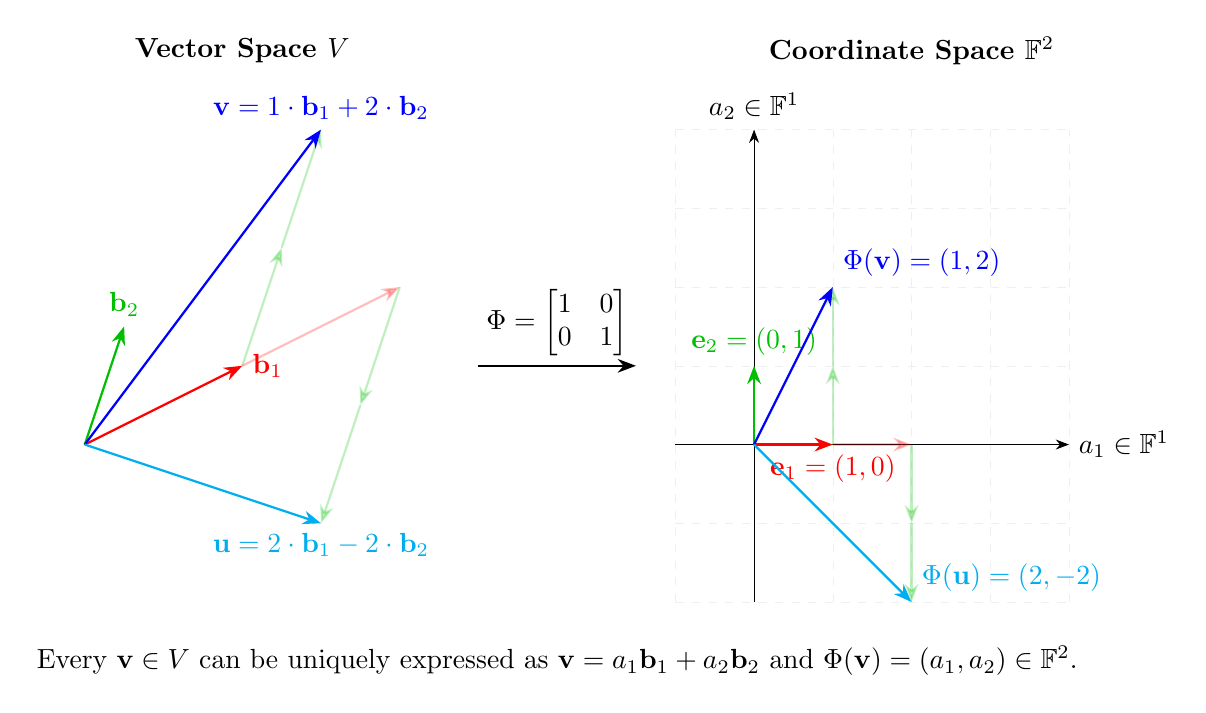
\begin{tikzpicture}[scale=1, >=Stealth]
	
	%%%%%%%%%%%%%%%%%%%%%%%%%%%%%%%%%%%%%%%%%%%%%%%%%%%%%%%%%%%%%%%%%%%%%%%%%%%%%%
	% Left Panel: Abstract Vector Space V
	%%%%%%%%%%%%%%%%%%%%%%%%%%%%%%%%%%%%%%%%%%%%%%%%%%%%%%%%%%%%%%%%%%%%%%%%%%%%%%
	\begin{scope}[shift={(-6,0)}]
		% Draw a grid for V (this grid is just to provide context)
%		\draw[step=1, gray!50, very thin, opacity=.5] (-1,-2) grid (4,4);
%		\draw[->] (-1,0) -- (4,0) node[right] {};
%		\draw[->] (0,-2) -- (0,4) node[above] {};
		\node at (2,5) {\textbf{Vector Space \(V\)}};
		
		% Define non-standard basis vectors of V:
		% Let v_1 = (2,0.5) and v_2 = (0.5,2)
		\draw[->, red, thick] (0,0) -- (2,1) node[anchor=west] {\(\vec{b}_1\)};
		\draw[->, green!75!black, thick] (0,0) -- (0.5,1.5) node[anchor=south] {\(\vec{b}_2\)};
		\draw[->, green!75!black, thick, opacity=.25] (2,1) -- (2.5,2.5) node[anchor=west] {};
		\draw[->, green!75!black, thick, opacity=.25] (2.5,2.5) -- (3,4) node[anchor=south] {};
		\draw[->, red, thick, opacity=.25] (2,1) -- (4,2) node[anchor=west] {};
		\draw[->, green!75!black, thick, opacity=.25] (4,2) -- (3.5,.5) node[anchor=west] {};
		\draw[->, green!75!black, thick, opacity=.25] (3.5,.5) -- (3,-1) node[anchor=west] {};
		
		% Draw an arbitrary vector v = a*v1 + b*v2, for example take a=1, b=2.
		% Then v = 1*(2,0.5) + 2*(0.5,2) = (2,0.5) + (1,4) = (3,4.5)
		\draw[->, blue, thick] (0,0) -- (3,4) node[anchor=south] {\(\vec{v}=1\cdot \vec{b}_1+2\cdot \vec{b}_2\)};
		\draw[->, cyan, thick] (0,0) -- (3,-1) node[anchor=north] {\(\vec{u}=2\cdot \vec{b}_1-2\cdot \vec{b}_2\)};
	\end{scope}
	
	%%%%%%%%%%%%%%%%%%%%%%%%%%%%%%%%%%%%%%%%%%%%%%%%%%%%%%%%%%%%%%%%%%%%%%%%%%%%%%
	% Middle: Mapping arrow representing \(\Phi\)
	%%%%%%%%%%%%%%%%%%%%%%%%%%%%%%%%%%%%%%%%%%%%%%%%%%%%%%%%%%%%%%%%%%%%%%%%%%%%%%
	\draw[->, thick] (-1,1) -- (1,1) node[midway, above] {\(\Phi=\begin{bmatrix}
			1 & 0 \\ 0 & 1
		\end{bmatrix}\)};
	
	%%%%%%%%%%%%%%%%%%%%%%%%%%%%%%%%%%%%%%%%%%%%%%%%%%%%%%%%%%%%%%%%%%%%%%%%%%%%%%
	% Right Panel: Coordinate Space \(F^2\)
	%%%%%%%%%%%%%%%%%%%%%%%%%%%%%%%%%%%%%%%%%%%%%%%%%%%%%%%%%%%%%%%%%%%%%%%%%%%%%%
	\begin{scope}[shift={(2.5,0)}]
		% Draw a standard grid for F^2 (using standard basis)
		\draw[step=1, gray!25, very thin, opacity=.5, dashed] (-1,-2) grid (4,4);
		\draw[->] (-1,0) -- (4,0) node[right] {\(a_1\in\F^1\)};
		\draw[->] (0,-2) -- (0,4) node[above] {$a_2\in\F^1$};
		\node at (2,5) {\textbf{Coordinate Space \(\F^2\)}};
		
		% In F^2, the standard basis vectors are:
		\draw[->, red, thick] (0,0) -- (1,0) node[anchor=north] {\(\vec{e}_1=(1,0)\)};
		\draw[->, green!75!black, thick] (0,0) -- (0,1) node[anchor=south] {\(\vec{e}_2=(0,1)\)};
		
		\draw[->, green!75!black, thick, opacity=.25] (1,0) -- (1,1) node[anchor=west] {};
		\draw[->, green!75!black, thick, opacity=.25] (1,1) -- (1,2) node[anchor=south] {};
		\draw[->, red, thick, opacity=.25] (1,0) -- (2,0) node[anchor=west] {};
		\draw[->, green!75!black, thick, opacity=.25] (2,0) -- (2,-1) node[anchor=west] {};
		\draw[->, green!75!black, thick, opacity=.25] (2,-1) -- (2,-2) node[anchor=west] {};
		
		% Under \Phi, the vector v becomes the coordinate vector (1,2)
		\draw[->, blue, thick] (0,0) -- (1,2) node[anchor=south west] {\(\Phi(\vec{v})=(1,2)\)};
		\draw[->, cyan, thick] (0,0) -- (2,-2) node[anchor=south west] {\(\Phi(\vec{u})=(2,-2)\)};
	\end{scope}
	
	%%%%%%%%%%%%%%%%%%%%%%%%%%%%%%%%%%%%%%%%%%%%%%%%%%%%%%%%%%%%%%%%%%%%%%%%%%%%%%
	% Bottom Annotation
	%%%%%%%%%%%%%%%%%%%%%%%%%%%%%%%%%%%%%%%%%%%%%%%%%%%%%%%%%%%%%%%%%%%%%%%%%%%%%%
	\node at (0,-2.75) {Every \(\vec{v}\in V\) can be uniquely expressed as \(\vec{v}=a_1\vec{b}_1+a_2\vec{b}_2\) and \(\Phi(\vec{v})=(a_1,a_2)\in \F^2\).};
	
\end{tikzpicture}
\end{center}
\vfill
Let \(V\) be an \(n\)-dimensional vector space over a field \(\F\). Suppose that \(\basis=\{\vec{b}_1, \vec{b}_2, \dots, \vec{b}_n\}\) is a basis of $V$ and that $\mathcal{E}=\set{\vec{e}_1,\vec{e}_2,\dots,\vec{e}_n}$ is a standard basis of $\F^n$. 
Define the mapping \[
\fullfunction{\Phi}{V}{\F^n}{\vec{v}}{\Phi(\vec{v})=\sum_{i=1}^{n}\alpha_i\vec{e}_i},
\] where $\vec{v}\in V$ is uniquely expressed as $\vec{v}=\sum_{i=1}^{n}\alpha_i\vec{b}_i$ with unique scalars $\set{\alpha_i}_{i=1}^n\subseteq\F$. Then 
\begin{align*}
	\Phi(\vec{b}_1)&=\Phi(1\cdot\vec{b}_1)=\vec{e}_1=1\vec{e}_1+0\vec{e}_2+\cdots+0\vec{e}_n,\\
	\Phi(\vec{b}_2)&=\Phi(1\cdot\vec{b}_2)=\vec{e}_2=0\vec{e}_1+1\vec{e}_2+\cdots+0\vec{e}_n,\\
	&\vdots \\
	\Phi(\vec{b}_n)&=\Phi(1\cdot\vec{b}_n)=\vec{e}_n=0\vec{e}_1+0\vec{e}_2+\cdots+1\vec{e}_n.
\end{align*}
Thus, the matrix representation of $\Phi$ w.r.t. the bases $\basis$ and $\mathcal{E}$ is the unique matrix \[
[\Phi]_{\basis}^{\mathcal{E}}=\begin{bmatrix}
	: & : & & : \\
	\Phi(\vec{b}_1) & \Phi(\vec{b}_2) & \cdots & \Phi(\vec{b}_n) \\
	: & : & & : \\
\end{bmatrix}=\begin{bmatrix}
1 & 0 & \cdots & 0\\
0 & 1 & \cdots & 0\\
\vdots & \vdots & \ddots &\vdots  \\
0 & 0 & \cdots & 1\\
\end{bmatrix}=:I_{n\times n}\ (\text{or just $I_n$}).
\] Hence each vector \(\vec{v} \in V\) is uniquely represented by its coordinate vector w.r.t. a fixed basis, thereby establishing an isomorphism.
\end{example*}

\newpage
\begin{example*}[Transpose Map]
Consider the vector space of \(2 \times 2\) matrices over \(\F\),
\[
\operatorname{Mat}_2(\F) = \left\{ \begin{bmatrix} a & b \\ c & d \end{bmatrix} \;:\; a,b,c,d \in \F \right\}.
\]
Define the mapping
\[
\Phi: \operatorname{Mat}_2(\F) \to \operatorname{Mat}_2(\F), \quad A=\begin{bmatrix} a & b \\ c & d \end{bmatrix} \mapsto A^T=\begin{bmatrix} a & c \\ b & d \end{bmatrix}.
\] Here $\Phi$ is linear: for any $A,B\in\text{Mat}_2(\F)$,
\[
\Phi(A+B) = (A+B)^T = A^T+B^T \quad\text{and}\quad \Phi(cA) = (cA)^T = cA^T.
\]
To express the matrix representation of \(\Phi\) w.r.t. a fixed basis, choose the standard basis for \(\operatorname{Mat}_2(\F)\):
\[\mathcal{E}=\set{
E_{11}=\begin{pmatrix}1&0\\0&0\end{pmatrix},\quad
E_{12}=\begin{pmatrix}0&1\\0&0\end{pmatrix},\quad
E_{21}=\begin{pmatrix}0&0\\1&0\end{pmatrix},\quad
E_{22}=\begin{pmatrix}0&0\\0&1\end{pmatrix}}.
\] Then \begin{align*}
	\Phi(E_{11})&=(E_{11})^T=E_{11}=1E_{11}+0E_{12}+0E_{21}+0E_{22},\\
	\Phi(E_{12})&=(E_{12})^T=E_{21}=0E_{11}+0E_{12}+1E_{21}+0E_{22},\\
	\Phi(E_{21})&=(E_{21})^T=E_{12}=0E_{11}+1E_{12}+0E_{21}+0E_{22},\\
	\Phi(E_{22})&=(E_{11})^T=E_{22}=0E_{11}+0E_{12}+0E_{21}+1E_{22}.
\end{align*} Thus, \[
[T]_{\mathcal{E}}^{\mathcal{E}}=\begin{bmatrix}
	: & : & : & : \\
	\Phi(E_{11}) & \Phi(E_{12}) & \Phi(E_{21}) & \Phi(E_{22}) \\
	: & : & : & : \\
\end{bmatrix}=\begin{bmatrix}
	1 & 0 & 0 & 0 \\
	0 & 0 & 1 & 0 \\
	0 & 1 & 0 & 0 \\
	0 & 0 & 0 & 1
\end{bmatrix}.
\]
\end{example*}
\vspace{20pt}
\begin{remark*}
The matrix representation of a linear transformation $T:V\to W$ is not canonical; it depends explicitly on the choices of bases for the domain $V$ and the codomain $W$.
\end{remark*}
\newpage
\begin{observation}
Let $V$ and $W$ be vector spaces over a field $\F$ with $\dim V=n$ and $\dim W=m$. Let $T:V\to W$ be a linear transformation. Suppose that \[
\basis_V=\set{\vec{v}_1,\vec{v}_2,\dots,\vec{v}_n}\quad\text{and}\quad\basis_W=\set{\vec{w}_1,\vec{w}_2,\dots,\vec{w}_n}
\] are bases for $V$ and $W$, respectively. See the following diagram:
\begin{center}
	\adjustbox{scale=1.25}{% https://tikzcd.yichuanshen.de/#N4Igdg9gJgpgziAXAbVABwnAlgFyxMJZABgBpiBdUkANwEMAbAVxiRADUQBfU9TXfIRQAWclVqMWbAOrdeIDNjwEiZYePrNWiEAB1dAWzo4AFgCMzwAGJcAeoR58lgoqPXVNUnfqOmL1uwNucRgoAHN4IlAAMwAnCCDEMhAcCCQARg9JbRAAFQBefQAFEywAfTB9AGMsWKqAAgBlatqG4tKyg1tgAFp0rjkY+MTk1KQAJiytNnbywmoGOjMYBiL+ZSEQWKwwkxwQamWwKCRkuFLo-cQAZkcQOISM6jGbqa89XRLyoOpzrEukNcFksVmtnCodNtdvs7g9EpMUmlXhJpjpGoVPh0DC06vVcji2pi5t0+gNYcMJs8kWcLlcgSj3rMKiT+gcQItlqt1i5ITs9oN7hTkS9Mgyckyur1Wb9aYDgZywQIIVs+TCKFwgA
		\begin{tikzcd}
			V \arrow[rrrr, "T=\Phi_n\circ S\circ \Phi_m^{-1}"] \arrow[dddd, "\Phi_n"', shift right=3]                 &  &  &  & W \arrow[dddd, "\Phi_m"', shift right=3]                 \\
			&  &  &  &                                                          \\
			&  &  &  &                                                          \\
			&  &  &  &                                                          \\
			\mathbb{F}^n \arrow[rrrr, "S=\Phi_m\circ T\circ \Phi_n^{-1}"] \arrow[uuuu, "\Phi_n^{-1}"', shift right=3] &  &  &  & \mathbb{F}^m \arrow[uuuu, "\Phi_m^{-1}"', shift right=3]
	\end{tikzcd}}
\end{center} Here $S:=\Phi_m\circ T\circ \Phi_n^{-1}$ is a linear transformation from $\F^n$ to $\F^m$. Suppose that $\mathcal{E}_n$ and $\mathcal{E}_m$ are the standard bases of $\F^n$ and $\F^m$, respectively. Then \begin{align*}
	[S]_{\mathcal{E}_n}^{\mathcal{E}_m} &= [\Phi_m\circ T\circ \Phi_n^{-1}]_{\mathcal{E}_n}^{\mathcal{E}_m}\\
	&=[\Phi_m]_{\basis_W}^{\mathcal{E}_m}[T]_{\basis_V}^{\basis_W}[\Phi_n^{-1}]_{\mathcal{E}_n}^{\basis_V}\\
	&=I_m[T]_{\basis_V}^{\basis_W}I_n\\
	&=[T]_{\basis_V}^{\basis_W}.
\end{align*}
\end{observation}\vspace{10pt}
\thmbox[Basis Change]{\begin{theorem*}
	TBA
\end{theorem*}}
\iffalse
\begin{observation}
Let $V$ and $W$ be vector spaces over a field $\F$ with $\dim V=n$ and $\dim W=m$. Let $T:V\to W$ be a linear transformation. Suppose that \[
\basis_V=\set{\vec{v}_1,\vec{v}_2,\dots,\vec{v}_n}\quad\text{and}\quad\basis_W=\set{\vec{w}_1,\vec{w}_2,\dots,\vec{w}_n}
\] are bases for $V$ and $W$, respectively. See the following diagram:
\begin{center}
\adjustbox{scale=1.25}{% https://tikzcd.yichuanshen.de/#N4Igdg9gJgpgziAXAbVABwnAlgFyxMJZABgBpiBdUkANwEMAbAVxiRADUQBfU9TXfIRQAWclVqMWbAOrdeIDNjwEiZYePrNWiEAB1dAWzo4AFgCMzwAGJcAeoR58lgoqPXVNUnfqOmL1uwNucRgoAHN4IlAAMwAnCCDEMhAcCCQARg9JbRAAFQBefQAFEywAfTB9AGMsWKqAAgBlatqG4tKyg1tgAFp0rjkY+MTk1KQAJiytNnbywmoGOjMYBiL+ZSEQWKwwkxwQamWwKCRkuFLo-cQAZkcQOISM6jGbqa89XRLyoOpzrEukNcFksVmtnCodNtdvs7g9EpMUmlXhJpjpGoVPh0DC06vVcji2pi5t0+gNYcMJs8kWcLlcgSj3rMKiT+gcQItlqt1i5ITs9oN7hTkS9Mgyckyur1Wb9aYDgZywQIIVs+TCKFwgA
\begin{tikzcd}
	V \arrow[rrrr, "T=\Phi_n\circ S\circ \Phi_m^{-1}"] \arrow[dddd, "\Phi_n"', shift right=3]                 &  &  &  & W \arrow[dddd, "\Phi_m"', shift right=3]                 \\
	&  &  &  &                                                          \\
	&  &  &  &                                                          \\
	&  &  &  &                                                          \\
	\mathbb{F}^n \arrow[rrrr, "S=\Phi_m\circ T\circ \Phi_n^{-1}"] \arrow[uuuu, "\Phi_n^{-1}"', shift right=3] &  &  &  & \mathbb{F}^m \arrow[uuuu, "\Phi_m^{-1}"', shift right=3]
\end{tikzcd}}
\end{center} Here $S:=\Phi_m\circ T\circ \Phi_n^{-1}$ is a linear transformation from $\F^n$ to $\F^m$. Suppose that $\mathcal{E}_n$ and $\mathcal{E}_m$ are the standard bases of $\F^n$ and $\F^m$, respectively. Then \begin{align*}
[S]_{\mathcal{E}_n}^{\mathcal{E}_m} &= [\Phi_m\circ T\circ \Phi_n^{-1}]_{\mathcal{E}_n}^{\mathcal{E}_m}\\
&=[\Phi_m]_{\basis_W}^{\mathcal{E}_m}[T]_{\basis_V}^{\basis_W}[\Phi_n^{-1}]_{\mathcal{E}_n}^{\basis_V}\\
&=I_m[T]_{\basis_V}^{\basis_W}I_n\\
&=[T]_{\basis_V}^{\basis_W}.
\end{align*}
\end{observation}
\begin{exercise*}
Let $V,W$ and $U$ be vector spaces over a field $\F$ with $\dim V=n$,\ $\dim W=m$ and $\dim W=l$. Let $T_1:V\to W$ and $T_2:W\to U$ are linear transformations. Then \[
T_2\circ T_1: V\to U
\]  is also a linear transformation. Let \begin{align*}
	\basis_V&=\set{\vec{v}_1,\vec{v}_2,\dots,\vec{v}_n},\\
	\basis_W&=\set{\vec{w}_1,\vec{w}_2,\dots,\vec{w}_m},\\
	\basis_U&=\set{\vec{u}_1,\vec{u}_2,\dots,\vec{u}_l}.
\end{align*} Then \[
[T_2\circ T_1]_{\basis_V}^{\basis_U}=[T_2]_{\basis_V}^{\basis_U}[T_1]_{\basis_W}^{\basis_V}.
\]
\end{exercise*}

\thmbox[Basis Change]{\begin{theorem*}
Let $V$ and $W$ be vector spaces over a field $F$. For a linear mapping $\Phi:V\to W$, bases \[
\basis_V=\set{\vec{v}_1,\dots,\vec{v}_n},\quad\tilde{\basis_V}=\set{\tilde{\vec{v}}_1,\cdots\tilde{\vec{v}}_n}
\] of \(V\) and 
\[
\basis_W=\set{\vec{w}_1,\dots,\vec{w}_n},\quad\tilde{\basis_W}=\set{\tilde{\vec{w}}_1,\cdots\tilde{\vec{w}}_n}
\] of \(W\), and a transformation matrix
% \(\textbf{A}_{\Phi}=\sbr[1]{a_{ij}}_{m\by n}\) w.r.t. \(\mathscr{B}\) and \(\mathscr{C}\), 
%the corresponding transformation matrix \(\tilde{\textbf{A}}_\Phi=\sbr[1]{\tilde{a}_{ij}}_{m\by n}\) w.r.t. the bases \(\tilde{\mathscr{B}}\) and \(\tilde{\mathscr{C}}\) is given
% \[
%\boxed{\tilde{\textbf{A}}_\Phi=\textbf{T}^{-1}\textbf{A}_\Phi \textbf{S}}.
%\]
%\begin{tikzcd}
%	&& V \arrow[rr, "\Phi"] && W && V \arrow[rr, "\Phi"] && W\\
%	&& \mathscr{B} \arrow[rr, "\textbf{A}_\Phi"] && \mathscr{C} && \mathscr{B} \arrow[rr, "\textbf{A}_\Phi"] && \mathscr{C} \arrow[dd, "\textbf{T}^{-1}"] \\
%	&& && && &&\\
%	&& \tilde{\mathscr{B}} \arrow[uu, "\textbf{S}"] \arrow[rr, "\tilde{\textbf{A}}_\Phi"] && \tilde{\mathscr{C}} \arrow[uu, "\textbf{T}"'] && \tilde{\mathscr{B}} \arrow[uu, "\textbf{S}"] \arrow[rr, "\tilde{\textbf{A}}_\Phi"] && \tilde{\mathscr{C}}             
%\end{tikzcd}	
\end{theorem*}}
\begin{proof}
%	Let \[
%	\textbf{S}:=\sbr[1]{s_{ij}}_{n\by n}=\sbr[2]{\tilde{\textbf{b}}_1\ \tilde{\textbf{b}}_2\ \cdots\ \tilde{\textbf{b}}_n}_{\basis},\quad
%	\text{and}\quad
%	\textbf{T}:=\sbr[1]{t_{lk}}_{m\by m}=\sbr[2]{\tilde{\textbf{c}}_1\ \tilde{\textbf{c}}_2\ \cdots\ \tilde{\textbf{c}}_m}_{\mathcal{C}}.
%	\] That is, \[
%	\tilde{\textbf{b}}_j=\begin{bmatrix}
%		s_{1j} \\ \vdots \\ s_{nj}
%	\end{bmatrix}_{\mathscr{B}}=\sum_{i=1}^ns_{ij}\textbf{b}_j\quad\text{and}\quad \tilde{\textbf{c}}_k=\begin{bmatrix}
%		t_{1k} \\ \vdots \\ t_{mk}
%	\end{bmatrix}_{\mathscr{C}}=\sum_{l=1}^mt_{lk}\textbf{c}_l
%	\] for $j=1,\dots,n$ and $k=1,\dots,m$, respectively. We must show that \[
%	\textbf{T}\tilde{\textbf{A}_\Phi}=\textbf{A}_\Phi\textbf{S}\in M_{m\by n}(\R).
%	\] \begin{enumerate}[(i)]
%		\item \((\textbf{T}\tilde{\textbf{A}_\Phi})\) For \(j=1,2,\dots,n\), \[
%		\Phi(\tilde{\textbf{b}}_j)=\sum_{k=1}^{m}\tilde{a}_{kj}\tilde{\textbf{c}}_k=\sum_{k=1}^m\sbr{\tilde{a}_{kj}\del{\sum_{l=1}^mt_{lk}\textbf{c}_l}}=\sum_{l=1}^m\sbr{\del{\sum_{k=1}^mt_{lk}\tilde{a}_{kj}}\textbf{c}_l}.
%		\]
%		\item \((\textbf{A}_\Phi\textbf{S})\) For \(j=1,2,\dots,n\), \[
%		\Phi(\tilde{\textbf{b}}_j)=\Phi\of{\sum_{i=1}^ns_{ij}\textbf{b}_j}=\sum_{i=1}^n\sbr{s_{ij}\Phi(\textbf{b}_i)}=\sum_{i=1}^n\sbr{s_{ij}\sum_{i=1}^ma_{li}\textbf{c}_l}=\sum_{l=1}^m\of{\sum_{i=1}^na_{li}s_{ij}}\textbf{c}_l.
%		\]
%	\end{enumerate}
	Hence \[
	\sum_{k=1}^mt_{lk}\tilde{a}_{kj}=\sum_{i=1}^na_{li}s_{ij}\implies\textbf{T}\tilde{\textbf{A}_\Phi}=\textbf{A}_\Phi\textbf{S}\implies\tilde{\textbf{A}}_\Phi=\textbf{T}^{-1}\textbf{A}_\Phi \textbf{S}.
	\]
\end{proof}

\probox{\begin{proposition*}
Let $V$ and $W$ be vector spaces over a field $\F$ with $\dim V=n$ and $\dim W=m$. Let $T:V\to W$ be a linear transformation. Suppose that \[
\basis_V=\set{\vec{v}_1,\vec{v}_2,\dots,\vec{v}_n}\quad\text{and}\quad\basis_W=\set{\vec{w}_1,\vec{w}_2,\dots,\vec{w}_n}
\] are bases for $V$ and $W$, respectively. Define a mapping \[
\fullfunction{\Phi}{\set{T\in (W^m)^{V^n}:T\ \text{is linear}}}{\operatorname{Mat}_{m\times n}(\F)}{T}{[T]_{\basis_V}^{\basis_W}}.
\] Then $\Phi$ be a bijection, \ie, there is an one-to-one correspondence between linear transformation and matrices.
\end{proposition*}}
\fi
\vfill
\begin{thebibliography}{9}
	\bibitem{linear_algebra_c}
	수학의 즐거움, Enjoying Math. ``수학 공부, 기초부터 대학원 수학까지, 16. 선형대수학 (c) 차원과 벡터공간의 분류'' YouTube Video, 29:08. Published 
	October 11, 2019. URL: \url{https://www.youtube.com/watch?v=rOKN645fRPs&t=399s}.
	\bibitem{linear_algebra_d}
	수학의 즐거움, Enjoying Math. ``수학 공부, 기초부터 대학원 수학까지, 17. 선형대수학 (d) 선형함수의 행렬 표현'' YouTube Video, 29:14. Published 
	October 12, 2019. URL: \url{https://www.youtube.com/watch?v=Fsy-9KW9-PA}.
\end{thebibliography}

\end{document}
